\begin{figure*}[t]
\centering
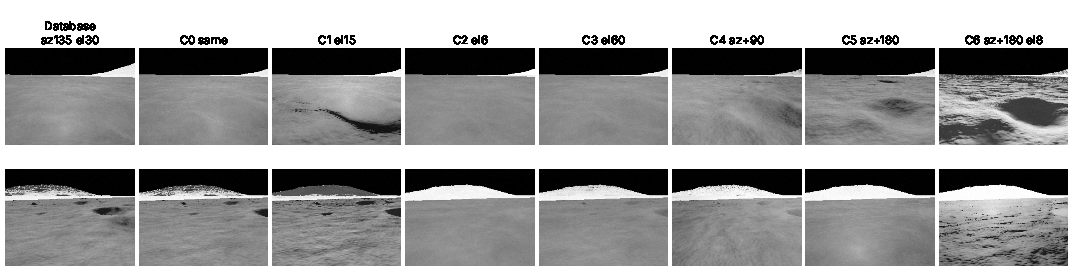
\includegraphics[width=\textwidth]{figures/conditions.pdf}
\caption{LunarSim-VPR: two test places (rows). Left: database image (Sun azimuth $135^\circ$,
elevation $30^\circ$). Right: queries at a jittered pose under the seven Sun conditions of
\cref{tab:conds}. Rendered with lunar-Lambert photometry, opposition surge and cast shadows from
local and regional relief. In the top row at C2, the camera lies in the shadow of a distant massif
and is lit only by the weak ambient term.}
\label{fig:conds}
\end{figure*}
\begin{figure}[t]
\centering
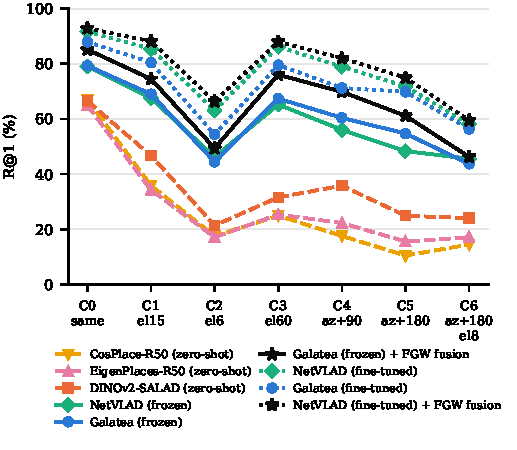
\includegraphics[width=\columnwidth]{figures/percond.pdf}
\caption{R@1 per illumination condition on the test set. Zero-shot terrestrial models (dashed)
collapse once the Sun moves. Lunar-trained OT aggregation (Galatea) and global--local fusion
(Galatea + FGW) recover much of the loss, most of all under shadow reversal and grazing light.}
\label{fig:percond}
\end{figure}
